\documentclass[12pt]{article}
\oddsidemargin   0mm
\evensidemargin  0mm
\topmargin       0mm
\headheight      0mm
\headsep         0mm
\topskip         0mm
\textwidth     160mm   % 210 - 25x2 mm
\textheight    235mm   % 297 - 30x2 -2 mm
\baselineskip  12pt    % single space  = 72.27pt / 6
\usepackage[dvips]{graphics}
\begin{document}
\pagestyle{empty}

%
%      FIGURE 1 : J0 Bessel Function
%
\begin{flushright} Fig.~1~:~ Kawano, T. (Kyushu U.) \end{flushright}
\vskip1cm
  \begin{center}
    \resizebox{150mm}{!}{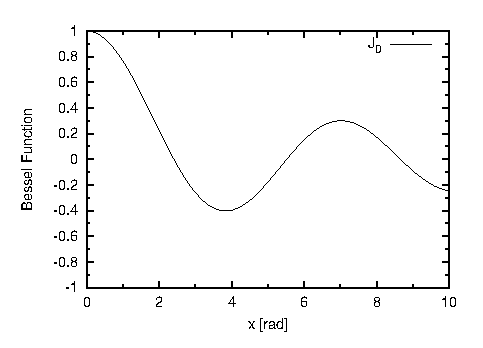
\includegraphics{besj0.eps}}
  \end{center}
\clearpage

%
%      FIGURE 2 : J1 Bessel Function
%
\begin{flushright} Fig.~2~:~ Kawano, T. (Kyushu U.) \end{flushright}
\vskip1cm
  \begin{center}
    \resizebox{150mm}{!}{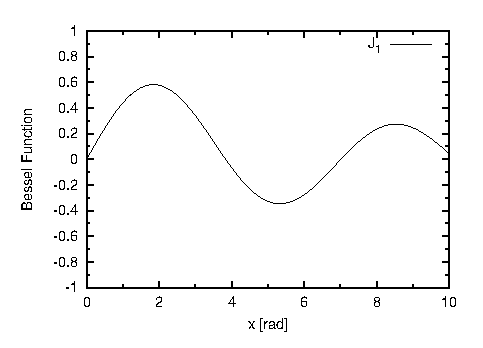
\includegraphics{besj1.eps}}
  \end{center}
\clearpage

%
%      FIGURE 3 : Y0 Bessel Function
%
\begin{flushright} Fig.~3~:~ Kawano, T. (Kyushu U.) \end{flushright}
\vskip1cm
  \begin{center}
    \resizebox{150mm}{!}{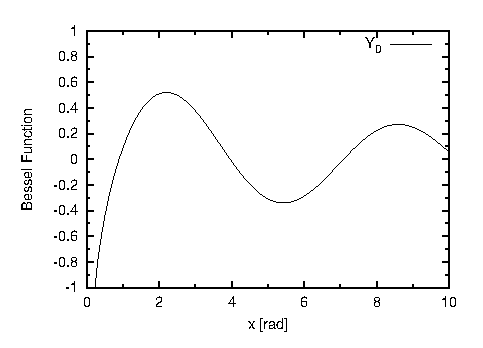
\includegraphics{besy0.eps}}
  \end{center}
\clearpage

%
%      FIGURE 4 : Y1 Bessel Function
%
\begin{flushright} Fig.~4~:~ Kawano, T. (Kyushu U.) \end{flushright}
\vskip1cm
  \begin{center}
    \resizebox{150mm}{!}{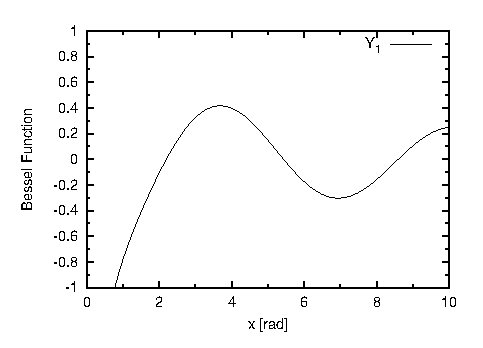
\includegraphics{besy1.eps}}
  \end{center}
\clearpage

%
%      FIGURE 5 : Bessel Functions
%
\begin{flushright} Fig.~5~:~ Kawano, T. (Kyushu U.) \end{flushright}
\vskip 1cm
\begin{center}
  \begin{tabular}{cc}
     \resizebox{70mm}{!}{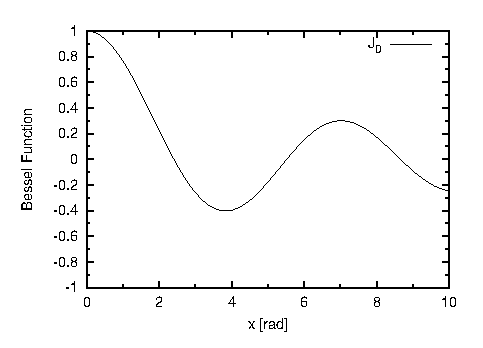
\includegraphics{besj0.eps}} &
     \resizebox{70mm}{!}{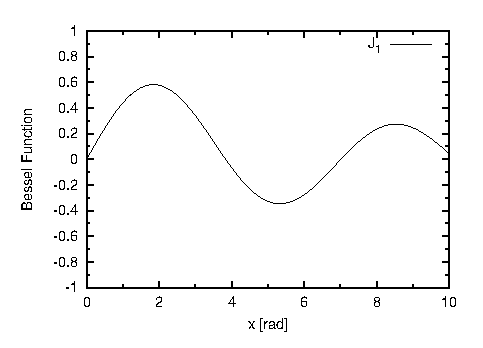
\includegraphics{besj1.eps}} \\
     \resizebox{70mm}{!}{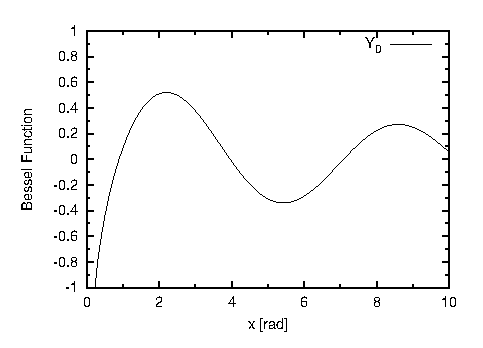
\includegraphics{besy0.eps}} &
     \resizebox{70mm}{!}{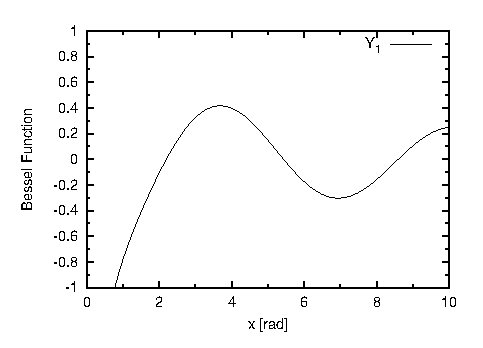
\includegraphics{besy1.eps}} \\
  \end{tabular}
\end{center}
\clearpage


%
%      FIGURE 6 : Y1 Bessel Function
%
\begin{flushright} Fig.~6~:~ Kawano, T. (Kyushu U.) \end{flushright}
\vskip1cm
  \begin{center}
    \rotatebox{90}{\resizebox{200mm}{!}{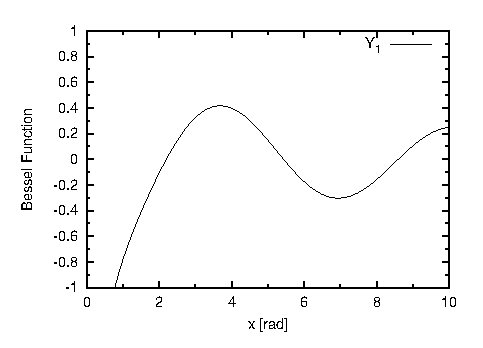
\includegraphics{besy1.eps}}}
  \end{center}
\clearpage

\end{document}
